%%%%%%%%%%%%%%%%%%%%%%%%%%%%%%%%%%%%%%%%%%%%%%%%%%%%%%%%%%%%%%%%%%%%%%
% Lớp 11 | Hàm số lượng giác và phương trình lượng giác | Giá trị lượng giác của một góc lượng giác
% Dạng 1D1?2-5: Toán thực tế áp dụng giá trị của một góc lượng giác
% Số câu: 14  (sinh tự động bởi tach_cau.py; từ nay thầy sửa trực tiếp file này)
%%%%%%%%%%%%%%%%%%%%%%%%%%%%%%%%%%%%%%%%%%%%%%%%%%%%%%%%%%%%%%%%%%%%%%

%%%%%%%%%%%%%%%% ĐÚNG/SAI %%%%%%%%%%%%%%%%

% nguồn: Ok_dungsai_lop11_Lan2
\begin{ex}%[1D1H2-5]%[ma:cdf22190]
	Cho $\cos \alpha=\dfrac{11}{61}$ và $-\dfrac{\pi}{2} < \alpha  < 0$.
	\choiceTF 
		 {$\sin \left(\dfrac{\pi}{6}-\alpha \right)=-\dfrac{60}{61}$}
		{\True $\cot \left(\alpha+\dfrac{\pi}{4} \right)=-\dfrac{71}{49}$} 
		{$\cos  \left(2\alpha+\dfrac{\pi}{3} \right)=\dfrac{\sqrt{3}}{2}$}
		{\True  $\tan \left(\dfrac{3\pi}{4}-2\alpha \right)=-\dfrac{4799}{2159}$}
	\loigiai{ 
		\begin{itemchoice}
			\itemch Vì $-\dfrac{\pi}{2} < \alpha <  0$ nên $\sin \alpha < 0$.\\
			Do đó  $\sin \alpha=-\sqrt{1-\cos ^2\alpha}=-\sqrt{1-\left(\dfrac{11}{61} \right)^2}=-\dfrac{60}{61}$.\\
			Suy ra $\sin \left(\dfrac{\pi}{6}-\alpha \right)=\sin \dfrac{\pi}{6} \cos \alpha-\cos \dfrac{\pi}{6} \sin \alpha=\dfrac{1}{2} \cdot \dfrac{11}{61}-\dfrac{\sqrt{3}}{2} \cdot \left(-\dfrac{60}{61} \right)=\dfrac{11+60\sqrt{3}}{122}$. 
			\itemch  Ta có $\tan \alpha=\dfrac{\sin \alpha}{\cos \alpha}=\dfrac{-\dfrac{60}{61}}{\dfrac{11}{61}}=-\dfrac{60}{11}$.\\
			 Do đó
			$\cot \left(\alpha+\dfrac{\pi}{4}\right)=\dfrac{1}{\tan  \left(\alpha+\dfrac{\pi}{4}\right)}=\dfrac{1-\tan \alpha \tan \dfrac{\pi}{4}}{\tan \alpha+\tan
			 \dfrac{\pi}{4}}=\dfrac{1-\left(-\dfrac{60}{11}\right) \cdot 1}{\left(-\dfrac{60}{11}\right)+1}=-\dfrac{71}{49}$.
			\itemch Ta có $\cos  2\alpha=2\cos ^2\alpha-1=2\cdot \left(\dfrac{11}{61} \right)^2-1=-\dfrac{3479}{3721}$.
			\\$ \sin 2\alpha=2\sin  \alpha \cos \alpha=2\cdot \left(-\dfrac{60}{61} \right)\cdot \dfrac{11}{61}=-\dfrac{1320}{3721}.$
			\begin{eqnarray*}
				\Rightarrow \cos \left(2\alpha+\dfrac{\pi}{3} \right)&=&\cos  2\alpha \cos \dfrac{\pi}{3}-\sin 2\alpha \sin \dfrac{\pi}{3}\\
				&=&-\dfrac{3479}{3721} \cdot  \dfrac{1}{2}-\left(-\dfrac{1320}{3721} \right)\cdot \dfrac{\sqrt{3}}{2}\\
				 &=&\dfrac{-3479+1320\sqrt{3}}{7442}.
			\end{eqnarray*}
			\itemch Ta  có
			\begin{eqnarray*}
				\tan 2\alpha&=&\dfrac{\sin  2\alpha}{\cos 2\alpha}=\dfrac{-\dfrac{1320}{3721}}{-\dfrac{3479}{3721}}\\
				 &=&\dfrac{1320}{3479}.
			\end{eqnarray*}
			 Suy ra
			\begin{eqnarray*}\tan \left(\dfrac{3\pi}{4}-2\alpha \right)&=&\dfrac{\tan \dfrac{3\pi}{4}-\tan 2\alpha}{1+\tan \dfrac{3\pi}{4} \tan 2\alpha}\\
				 &=&\dfrac{-1-\dfrac{1320}{3479}}{1+\left(-1\right)\cdot \dfrac{1320}{3479}}\\
				&=&-\dfrac{4799}{2159}. 
			\end{eqnarray*}
		\end{itemchoice}
	 }
\end{ex}

% nguồn: Ok_dungsai_lop11_Lan2
\begin{ex}%[1D1H2-5]%[ma:2ef5adc2]
	Xét tính đúng - sai của các khẳng định sau đây. 
	\choiceTF 
		{\True $\sin \dfrac{19\pi}{24} \cos  \dfrac{37\pi}{24}=\dfrac{\sqrt{3}-\sqrt{2}}{4}$}
		{$\cos \dfrac{41\pi}{12}-\cos \dfrac{13\pi}{12}=\sqrt{2}$} 
		{$\dfrac{\tan \dfrac{\pi}{7}+\tan \dfrac{3\pi}{28}}{1+\tan \dfrac{6\pi}{7} \tan \dfrac{3\pi}{28}}=2$} 
		{\True $\sin  \dfrac{\pi}{9}-\sin \dfrac{5\pi}{9}+\sin \dfrac{7\pi}{9}=0$}
	\loigiai{ 
		\begin{itemchoice}
			 \itemch
			\begin{eqnarray*}
				 &&\sin \dfrac{19\pi}{24} \cos \dfrac{37\pi}{24}\\
				&=&\dfrac{1}{2}  \left[\sin \left(\dfrac{19\pi}{24}-\dfrac{37\pi}{24} \right)+\sin \left(\dfrac{19\pi}{24}+\dfrac{37\pi}{24} \right)\right]\\
				& = &  \dfrac{1}{2} \left(- \sin\dfrac{3\pi }{4} + \sin \dfrac{7\pi }{3} \right)\\
				& = & \dfrac{1}{2}\left[- \sin \dfrac{3\pi }{4} + \sin\left( \dfrac{\pi }{3} + 2 \pi  \right)\right]\\
				&=& \dfrac{1}{2} \left( - \sin \dfrac{3\pi }{4}+ \sin \dfrac{\pi }{3}\right)\\ 
				 & = & \dfrac{\sqrt{3}-\sqrt{2}}{4}.
			\end{eqnarray*}
			\itemch Ta có 
			\begin{eqnarray*}
				 \cos \dfrac{41\pi}{12}-\cos \dfrac{13\pi}{12}&=&-2\sin \dfrac{\dfrac{41\pi}{12}+\dfrac{13\pi}{12}}{2} \sin \dfrac{\dfrac{41\pi}{12}-\dfrac{13\pi}{12}}{2}\\
				&=&-2\sin \dfrac{9\pi}{4} \sin \dfrac{7\pi}{6} 
				 \\&=&2\sin \dfrac{\pi}{4} \sin \dfrac{\pi}{6}
				\\&=&2\cdot \dfrac{\sqrt{2}}{2} \cdot  \dfrac{1}{2}\\
				 &=&\dfrac{\sqrt{2}}{2}.
			\end{eqnarray*}
			\itemch  Ta có
			\begin{eqnarray*}\dfrac{\tan \dfrac{\pi}{7}+\tan \dfrac{3\pi}{28}}{1+\tan \dfrac{6\pi}{7} \tan \dfrac{3\pi}{28}}&=&\dfrac{\tan \dfrac{\pi}{7}+\tan \dfrac{3\pi}{28}}{1+\tan \left(\pi-\dfrac{\pi}{7} \right)\tan \dfrac{3\pi}{28}}\\
				&=&\dfrac{\tan \dfrac{\pi}{7}+\tan \dfrac{3\pi}{28}}{1-\tan \dfrac{\pi}{7} \tan  \dfrac{3\pi}{28}}\\
				&=&\tan  \left(\dfrac{\pi}{7}+\dfrac{3\pi}{28} \right)\\
				&=&\tan  \dfrac{\pi}{4}=1.
			\end{eqnarray*}
			\itemch Ta  có
			\begin{eqnarray*} \sin \dfrac{\pi}{9}-\sin \dfrac{5\pi}{9}+\sin \dfrac{7\pi}{9}&=&\left(\sin \dfrac{\pi}{9}+\sin \dfrac{7\pi}{9} \right)-\sin \dfrac{5\pi}{9}\\
				&=&2\sin \dfrac{4\pi}{9} \cdot \cos  \dfrac{\pi}{3}-\sin \dfrac{5\pi}{9}\\
				 &=&\sin \dfrac{4\pi}{9}-\sin \dfrac{5\pi}{9}=0.
			\end{eqnarray*}
		\end{itemchoice}
	 }
\end{ex}

% nguồn: Ok_dungsai_lop11_Lan2
\begin{ex}%[1D1H2-5]%[ma:d9028f45]
	 Xét tính đúng sai của các khẳng định sau.
	 \choiceTF
		 {$\sin x\cos ^5x-\cos x\sin ^5x=\sin 4x$}
		{$\dfrac{\sin 3x\cos  2x+\sin x\cos 6x}{\sin 4x}=\cos3x$;}
		{$\dfrac{\cos x-\cos 2x+\cos 3x}{\sin x-\sin 2x+\sin  3x}=\cot 2x$}
		{$\dfrac{2\sin \left(x+y\right)}{\cos \left(x+y\right)+\cos  \left(x-y\right)}-\tan y=1$}
	\loigiai{ 
		\begin{itemchoice}
			\itemch 
			\begin{eqnarray*}
				\sin  x\cos ^5x-\cos x\sin ^5x&=&\sin x\cos x\left(\cos ^4x-\sin ^4x\right)
				\\ 
				&=&\dfrac{1}{2} \sin 2x\left(\cos  ^2x-\sin ^2x\right)\left(\cos ^2x+\sin ^2x\right)\\
				&=&\dfrac{1}{2} \sin 2x\cos  2x=\dfrac{1}{4} \sin 4x.
			\end{eqnarray*}
			 \itemch Ta có
			\begin{eqnarray*}\dfrac{\sin 3x\cos 2x+\sin x\cos 6x}{\sin 4x}&=&\dfrac{\dfrac{1}{2} \left(\sin x+\sin 5x\right)+\dfrac{1}{2} \left[\sin \left(-5x\right)+\sin 7x\right]}{\sin 4x}\\
				&=&\dfrac{\sin x+\sin  5x-\sin 5x+\sin 7x}{2\sin 4x}\\
				&=&\dfrac{\sin x+\sin 7x}{2\sin 4x}\\ 
				 &=&\dfrac{2\sin 4x\cos 3x}{2\sin 4x}\\
				&=&\cos 3x. 
			\end{eqnarray*}
			\itemch 
			\begin{eqnarray*}\dfrac{\cos x-\cos 2x+\cos 3x}{\sin x-\sin 2x+\sin 3x}&=&\dfrac{\left(\cos x+\cos 3x\right)-\cos 2x}{\left(\sin x+\sin 3x\right)-\sin 2x}\\
				&=&\dfrac{2\cos 2x\cos x-\cos 2x}{2\sin 2x\cos  x-\sin 2x}\\
				&=&\dfrac{\cos 2x\left(2\cos x-1\right)}{\sin 2x\left(2\cos  x-1\right)}\\
				 &=&\dfrac{\cos 2x}{\sin 2x}=\cot 2x.
			\end{eqnarray*}
			\itemch 
			\begin{eqnarray*}
				\dfrac{2\sin \left(x+y\right)}{\cos \left(x+y\right)+\cos \left(x-y\right)}-\tan y&=&\dfrac{2\left(\sin x\cos y+\cos x\sin y\right)}{2\cos x\cos y}-\tan  y\\
				&=&\dfrac{\sin x}{\cos x}+\dfrac{\sin  y}{\cos y}-\tan y\\
				&=&\tan x+\tan y-\tan y=\tan  x.
			\end{eqnarray*}
		\end{itemchoice}
	} 
\end{ex}

% nguồn: Ok_dungsai_lop11_Lan1
\begin{ex}%[1D1V2-5]%[ma:4194aaa3]
 Từ một vị trí ban đầu trong không gian, vệ tinh $X$ chuyển động theo quỹ đạo là một đường tròn quanh Trái Đất và luôn cách tâm Trái Đất một khoảng bằng $9200$ km. Sau 2 giờ thì vệ tinh $X$ hoàn thành hết một vòng  di chuyển. Các khẳng định sau đây đúng hay sai?
  \choiceTF
  {\True Quãng đường vệ tinh $X$ chuyển động được sau $1$ giờ là  $\approx 28902{,}65$ (km)}
  {\True Quãng đường vệ tinh $X$ chuyển động được sau  $1{,}5$ giờ là $\approx 43353{,}98$ (km)}
  {Sau khoảng 5,3 giờ thì $X$ di chuyển được  quãng đường $240000$ (km)}
  {\True Giả sử vệ tinh di chuyển theo chiều dương của đường tròn, sau $4{,}5$ giờ thì vệ tinh vẽ nên một góc  $\dfrac{9\pi}{2}$ rad}
 \loigiai{ 
  \begin{itemchoice}
   \itemch Một vòng di  chuyển của $X$ chính là chu vi đường tròn\\
   \centerline{$C=2\pi R=2\pi .9200=18400\pi$  (km).}\\
   Sau 1 giờ, vệ tinh di chuyển nửa đường tròn với quãng đường là \\ 
   \centerline{$\dfrac{1}{2}C=9200\pi\approx 28902,65$ (km).} 
   \itemch Sau 1,5 giờ, vệ tinh di chuyển được  $\dfrac{1,5.1}{2}$ đường tròn (hay $\dfrac{3}{4}$ đường tròn), quãng đường là\\ \centerline{$\dfrac{3}{4}C=\dfrac{3}{4}\cdot 18400\pi=13800\pi\approx 43353,98$ (km).}
    \itemch Số giờ để vệ tinh $X$ thực hiện quãng đường $240000$ km là $\dfrac{240000}{9200\pi}\approx 8,3$ (giờ).
   \itemch Sau $4{,}5$ giờ thì số vòng tròn mà  vệ tinh $X$ di chuyển được là $\dfrac{4{,}5}{2}=\dfrac{9}{4}$ (vòng).
   \itemch Số đo góc lượng giác thu được là  $\dfrac{9}{4}\cdot 2\pi=\dfrac{9\pi}{2}$ (rad).
  \end{itemchoice}
 } 
\end{ex}

% nguồn: Ok_dungsai_lop11_Lan2
\begin{ex}%[1D1V2-5]%[ma:3647f24b]
	Từ một vị  trí ban đầu trong không gian, vệ tinh $X$ chuyển động theo quỹ đạo là một đường tròn quanh Trái Đất và luôn cách tâm Trái Đất một khoảng bằng $9\,200$ km. Sau $2$ giờ thì vệ tinh $X$ hoàn thành hết một vòng di chuyển.
	 \choiceTF
		{\True Quãng đường vệ tinh $X$ chuyển động được sau $1$ giờ là  $28\,902{,}65$ km (làm tròn đến hàng phần trăm)}
		{\True Quãng đường vệ tinh $X$ chuyển động được sau $1{,}5$ giờ là  $43\,353{,}98$ km (làm tròn đến hàng phần trăm)}
		{Sau khoảng $5{,}3$ giờ thì $X$ di chuyển được quãng  đường $240\,000$ km}
		{\True Giả sử vệ tinh di chuyển theo chiều dương của đường tròn, sau $4{,}5$ giờ thì vệ tinh vẽ nên một  góc $\dfrac{9\pi}{2}$ rad}
	 \loigiai{
		\begin{itemchoice}
			\itemch \textbf{Đúng}.\\  Một vòng di chuyển của $X$ chính là chu vi đường tròn
			$C=2\pi R=2\pi \cdot 9\,200=18\,400\pi$ (km) 
			Sau $1$ giờ, vệ tinh di chuyển nửa đường tròn với  quãng đường là
			 $\dfrac{1}{2} C=9\,200\pi \approx 28\,902{,}65$ (km).
			\itemch \textbf{Đúng}.\\ Sau $1{,}5$ giờ, vệ tinh di chuyển được $\dfrac{1{,}5 \cdot 1}{2}$ đường tròn (hay $\dfrac{3}{4}$ đường  tròn), quãng đường là $\dfrac{3}{4} C=\dfrac{3}{4} \cdot 18\,400\pi=13\,800\pi \approx 43\,353{,}98$ km.
			\itemch \textbf{Sai}.\\  Số giờ để vệ tinh $X$ thực hiện quãng đường $240\,000$ km là $\dfrac{240\,000}{9\,200\pi} \approx 8{,}3$ (giờ)
			\itemch \textbf{Đúng}.\\ Sau  $4{,}5$ giờ thì số vòng tròn mà vệ tinh $X$ di chuyển được là $\dfrac{4{,}5}{2}=\dfrac{9}{4}$ (vòng)\\
			Số đo góc lượng giác  thu được là $\dfrac{9}{4} \cdot 2\pi=\dfrac{9\pi}{2}$ (rad).
	\end{itemchoice}}
\end{ex}


%%%%%%%%%%%%%%%% TRẢ LỜI NGẮN %%%%%%%%%%%%%%%%

% nguồn: Ok_TraLoiNgan_Lop11_Lan2
\begin{ex}%[1D1H2-5]%[ma:0d5ac4c9]
	Trạm vũ rụ Quốc tế ISS nằm trong quỹ đạo tròn cách bề mặt trái Trái Đất khoảng $400$ km. Nếu trạm mặt đất theo dõi được trạm vũ trụ ISS khi nó nằm trong góc $60^\circ$ ở tâm của quỹ đạo tròn này phía trên ăng – ten theo dõi, thì trạm vũ  trụ ISS đã di chuyển được bao nhiêu kilômét (làm tròn tới hàng đơn vị) trong khi nó đang được trạm mặt đất theo dõi? Giả sử rằng đường kính trái đất là $12\,800$ km.
	\shortans{7,12} 
	\loigiai{ 
		 Bán kính quỹ đạo của trạm vũ trụ quốc tế là $R=6\,400+400=6\,800$ km.\\
		Đổi $60^\circ=60 \cdot \dfrac{\pi}{180}=\dfrac{\pi}{3}$.\\ 
		Vậy khi được trạm mặt đất theo dõi, trạm ISS đã di  chuyển quãng đường là
		$l=6\,800\cdot\dfrac{\pi}{3}\approx  7\,121$ km.
	} 
\end{ex}

% nguồn: Ok_TraLoiNgan_Lop11_Lan2
\begin{ex}%[1D1H2-5]%[ma:d33d609e]
	Một vệ tinh được định vị tại vị trí $A$ trong không gian. Từ vị trí $A$, vệ tinh bắt đầu chuyển động quanh Trái Đất theo quý đạo là đường tròn với tâm là tâm $O$ của tái đất và bán kính $9\,000$ km. Biết vệ tinh chuyển động hết một vòng của quỹ đạo trong $2$ giờ. Hỏi vệ  tịnh chuyển động quãng đường $300\,000$ km sau bao nhiêu giờ (làm tròn kết quả đến hàng phần trăm)?
	\shortans{10,6} 
	 \loigiai{
		Mỗi giờ vệ tinh đi được quãng đường là $\dfrac{1}{2} \cdot 2\pi \cdot 9\,000=9\,000\pi$ km.\\ 
		Để vệ tinh đi được quãng đường $300\,000$ km cần  đi thời gian là $\dfrac{300\,000}{9\,000\pi}\approx 10{,}61$ giờ.
	} 
\end{ex}

% nguồn: Ok_TraLoiNgan_Lop11_Lan2
\begin{ex}%[1D1H2-5]%[ma:301e15e0]
	Một máy kéo nông nghiệp với bánh  xe sau có đường kính là $192$ cm, bánh xe trước có đường kính là $96$ cm, xe chuyển động với vận tốc không đổi trên một đoạn đường thẳng. Biết vận tốc của bánh xe trước là $150$ vòng/phút. Tính vận tốc bánh xe trước (theo đơn vị vòng/phút).
	\shortans{75} 
	 \loigiai{
		Trong vòng $1$  phút bánh xe trước quay một góc $150 \cdot 2\pi=300\pi$ rad.\\
		Trong vòng $1$  phút máy kéo đi được quãng đường là $S=300\pi \cdot 96=28800\pi$ cm.\\
		Suy ra trong vòng $1$ phút bánh xe  sau quay một góc $150\pi$.\\
		Vậy  vận tốc của bánh xe sau là $\dfrac{150\pi}{2\pi}=75$ vòng/phút.
	} 
\end{ex}

% nguồn: Ok_TraLoiNgan_Lop11_Lan2
\begin{ex}%[1D1H2-5]%[ma:535d21a8]
	Độ dài của ngày từ lúc Mặt Trời mọc đến lúc Mặt Trời lặn ở một thành phố $X$ trong  ngày thứ $t$ của năm được tính xấp xỉ bởi công thức $d(t)=4\sin\left[\dfrac{2\pi }{365} (t-80)\right]+12\,\, (t\in \mathbb{Z}$ và $1\le t\le 365)$. Thành phố $X$ vào ngày $31$ tháng $1$ có bao nhiêu giờ có Mặt Trời chiếu sáng? (\textit{Kết quả làm tròn đến hàng phần trăm}).
	\shortans{9,01} 
	\loigiai{ 
		 Ta có $d(31)=9{,}01$ giờ.
	} 
\end{ex}

% nguồn: Ok_TraLoiNgan_Lop11_Lan1
\begin{ex}%[1D1V2-5]%[ma:7f657634]
	Trong thực tế, người ta có sử dụng lượng giác trong việc sử dụng GPS để kiểm tra vị trí của vệ tinh từ tọa độ trên Trái Đất. Cho $ f(x) = 26\,750 \cos x\cos(\pi-x)$ (km); $g(x)=26\,750\cos x\sin(\pi-x)$ (km); $h(x)=26\,750\sin x$ (km) ($x$ tính theo đơn vị radian) lần lượt là vị trí tọa độ của vệ tinh xác định trong không gian thay đổi theo tọa độ $x$ trên Trái Đất. Khi vị trí trên Trái Đất ở điểm $x=30^\circ$ thì vị trí của vệ tinh sẽ được biểu thị dưới dạng tọa độ là $(a;b;c)$, với $a=f(x),b=g(x),c=h(x)$. Khi đó giá trị của biểu thức $P=\dfrac{a-b+c}{100}$ là bao nhiêu (làm tròn kết quả đến hàng đơn  vị)?
	\shortans{-183} 
	 \loigiai{
		 Ta có $30^\circ=\dfrac{\pi}{6}$.\\
		$a=f\left(\dfrac{\pi}{6}\right)=  26\,750 \cos\left(\dfrac{\pi}{6}\right)\cos\left(\pi-\dfrac{\pi}{6}\right)=-20\,062{,}5$.\\[2mm]
		$b=g\left(\dfrac{\pi}{6}\right)=26\,750\cos\left(\dfrac{\pi}{6}\right)\sin\left(\pi-\dfrac{\pi}{6}\right)=\dfrac{13\,375\sqrt{3}}{2}$.\\[2mm] 
		 $c=h\left(\dfrac{\pi}{6}\right)=26\,750\sin\left(\dfrac{\pi}{6}\right)=13\,375$.\\[2mm]
		$P=\dfrac{a-b+c}{100}=\dfrac{-20\,062{,}5-\dfrac{13\,375\sqrt{3}}{2}+13\,375}{100}\approx  -183$.
	 }
\end{ex}

% nguồn: Ok_TraLoiNgan_Lop11_Lan1
\begin{ex}%[1D1V2-5]%[ma:976a93fb]
	Một người đi xe đạp đã đi được quãng đường $494{,}8$ m trong thời gian $2$ phút. Biết rằng đường kính bánh xe là $700$ mm. Hỏi trong $3$ giây bánh xe quay được  một góc lượng giác có số đo (đơn vị Radian) là bao nhiêu (giả sử bánh xe quay theo chiều dương, kết quả làm tròn đến một chữ số sau dấu phẩy)?
	\shortans{35,3} 
	\loigiai{ 
		Đổi đơn  vị: $700$ mm $=0{,}7$ m.\\
		Chu vi bánh xe là $C=2\pi r=0{,}7\pi $  m.\\
		Trong 2 phút  bánh xe quay được số vòng là: $n=\dfrac{494{,}8}{0{,}7\pi }\approx 225$ (vòng).\\
	Mỗi vòng bánh xe đã quay được một góc $360^\circ$ tương ứng với $2\pi $  (radian) nên trong $3$ giây bánh xe đã quay được góc lượng giác có số đo là $\alpha =\dfrac{3}{120}\cdot \dfrac{4948}{7\pi }\cdot 2\pi =35{,}3$ (rad).}
\end{ex}

% nguồn: Ok_TraLoiNgan_Lop11_Lan2
\begin{ex}%[1D1V2-5]%[ma:941ece95]
	\immini{	Từ một vị trí $A$, người ta buộc hai sợi cáp $AB$ và $AC$ đến một cái trụ cao $15\; m$, được dựng vuông góc với mặt đất, chân trụ ở vị trí $D$. Biết $CD=9$ mét và $AD=12$ mét. Tìm góc nhọn $\alpha=\widehat{BAC}$ tạo bởi hai sợi dây cáp đó, đồng thời tính gần đúng $\alpha$ (làm tròn đến hàng phần chục, đơn vị độ).}{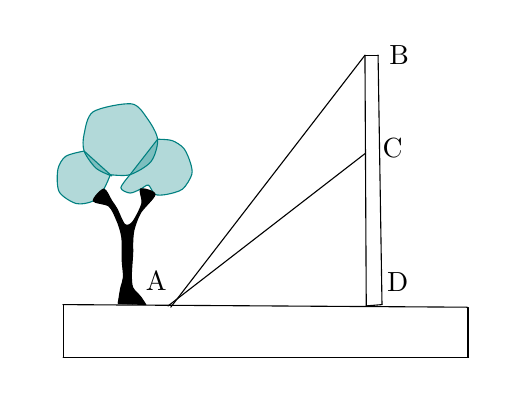
\begin{tikzpicture}[line join=round,line cap=round,>=stealth,scale=0.5]
		\definecolor{mycolor1}{rgb}{0.000,0.502,0.502} 
		\path[use as bounding box] (-6.367,-4.800)  rectangle (5.633,4.267);
		 \draw (-5.467,-2.767) rectangle (-5.467,-4.100);
		 \draw (4.833,-4.100) rectangle (4.800,-2.833);
		\draw (-5.467,-2.767) rectangle (-5.467,-2.767); 
		\filldraw (4.833,-4.100) rectangle  (-5.467,-4.100);
		 \draw (-2.733,-2.833) -- (2.200,3.567);
		\draw (2.200,3.567) --  (2.533,3.567);
		\filldraw[mycolor1,fill=mycolor1,fill opacity=0.3] plot[smooth]  coordinates{(-4.233,0.500)
			 (-4.633,0.700)
			 (-4.933,1.133)
			(-4.933,1.567) 
			 (-4.700,2.133)
			(-3.733,2.333) 
			(-3.333,1.967) 
			 (-3.067,1.433)
			(-3.233,0.867) 
			 (-3.767,0.533)
			(-4.267,0.533)}  -- cycle;
		\filldraw[mycolor1,fill=mycolor1,fill opacity=0.3] plot[smooth] coordinates{(-4.933,1.133) 
			 (-5.400,1.000)
			 (-5.600,0.667)
			(-5.567,0.100) 
			(-5.133,-0.200) 
			 (-4.700,-0.133)
			 (-4.433,0.167)
			(-4.267,0.533)} --  cycle;
		\filldraw[mycolor1,fill=mycolor1,fill opacity=0.3] plot[smooth] coordinates{(-3.767,0.533) 
			 (-4.000,0.200)
			 (-3.767,0.067)
			(-3.500,0.167) 
			 (-3.300,0.267)
			 (-3.133,0.033)
			(-2.833,0.033) 
			 (-2.433,0.167)
			 (-2.200,0.533)
			 (-2.233,0.833)
			(-2.400,1.200) 
			(-2.700,1.400) 
			 (-3.067,1.433)} -- cycle;
		\filldraw plot[smooth] coordinates{(-4.067,-2.733) 
			(-4.000,-2.333) 
			(-3.933,-2.067) 
			 (-3.967,-1.633)
			(-3.967,-1.167) 
			(-4.000,-0.933) 
			 (-4.100,-0.633)
			 (-4.300,-0.267)
			(-4.700,-0.133) 
			(-4.433,0.167) 
			 (-4.233,-0.133)
			 (-4.100,-0.333)
			 (-3.900,-0.733)
			 (-3.700,-0.667)
			 (-3.467,-0.200)
			 (-3.500,0.167)
			(-3.133,0.033) 
			(-3.500,-0.433) 
			 (-3.667,-0.867)
			(-3.700,-1.200) 
			(-3.700,-1.467) 
			(-3.733,-2.000) 
			(-3.700,-2.333) 
			 (-3.500,-2.567)
			(-3.367,-2.767)}  -- cycle;
		\draw (-5.467,-2.767) -- (4.800,-2.833); 
		\draw (-2.800,-2.800) -- (2.200,1.067); 
		 \draw (2.200,3.567) -- (2.233,-2.800);
		\draw (2.233,-2.800)  -- (2.633,-2.767);
		\draw (2.533,3.567) -- (2.533,3.567); 
		\draw (2.633,-2.767)  -- (2.533,3.567);
		\node  (node5) at (-3.100,-2.167) {A};
		\node  (node7) at (3.067,3.567) {B};
		 \node (node8) at (2.900,1.200) {C};
		\node (node9) at  (3.033,-2.2) {D};
	\end{tikzpicture}
	}\shortans{14,5} 
	 \loigiai{
		Ta có: $\tan \alpha=\tan \left(\widehat{BAD}-\widehat{CAD}\right)=\dfrac{\tan \widehat{BAD}-\tan  \widehat{CAD}}{1+\tan \widehat{BAD}\tan \widehat{CAD}}=\dfrac{\dfrac{15}{12}-\dfrac{9}{12}}{1+\dfrac{15}{12} \cdot \dfrac{9}{12}}=\dfrac{8}{31}.$\\
		Vậy $\alpha \approx 14{,}5^{\circ}$. 
	} 
\end{ex}

% nguồn: Ok_TraLoiNgan_Lop11_Lan2
\begin{ex}%[1D1V2-5]%[ma:c948ef31]
	\immini{	Trên một mảnh đất hình vuông $ABCD$ bác An đặt một chiếc đèn pintại vị trí $A$ chiếu chùm sáng phân kì sang phía góc $C$. Bác An nhận thấy góc chiếu sáng của đèn pin giới hạn bởi hai tia $AM$ và $AN$ mà ở đó các điểm $M\in BC; N\in DC$ sao cho $BM=\dfrac{1}{2} BC,DN=\dfrac{1}{3} DC$. Góc chiếu sáng của đèn pin bằng bao nhiêu độ?}{\begin{tikzpicture}[scale=0.6,font=\footnotesize,line join=round,line cap=round,>=stealth]
		\coordinate (A)  at (0,0);
		\coordinate (B)  at ($(A)+(0:5)$);
		\coordinate (C)  at ($(B)+(-90:5)$);
		 \coordinate (D) at ($(A)+(-90:5)$);
		\coordinate  (M) at ($(B)!1/2!(C)$);
		\coordinate (N)  at ($(D)!1/3!(C)$);
		 \draw (A)--(B)--(C)--(D)--cycle (M)--(A)--(N);
		\foreach \p/\r  in {A/180,B/90,C/0,D/180,M/0,N/-90}
		 \fill (\p) circle (1.5pt) node[shift={(\r:3mm)}]{$\p$};
	\end{tikzpicture}
	}\shortans{45} 
	\loigiai{ 
		Trong  tam giác vuông $ABM,\tan \widehat{BAM}=\dfrac{BM}{BA}=\dfrac{1}{2}$.\\
		 Trong tam giác vuông $ADN$, $\tan \widehat{DAN}=\dfrac{DN}{DA}=\dfrac{1}{3}$.\\
		 Do đó $\tan \left(\widehat{BAM}+\widehat{DAN}\right)=\dfrac{\tan \widehat{BAM}+\tan \widehat{DAN}}{1-\tan \widehat{BAM}\tan \widehat{DAN}}=\dfrac{\dfrac{1}{2}+\dfrac{1}{3}}{1-\dfrac{1}{2} \cdot \dfrac{1}{3}}=1$.\\
		Do $\tan  \left(\widehat{BAM}+\widehat{DAN}\right)=1$ nên $\widehat{BAM}+\widehat{DAN}=45^{\circ}.$\\ Suy ra $\widehat{MAN}=90^{\circ}-\left(\widehat{BAM}+\widehat{DAN}\right)=45^{\circ}$.\\
		 Vậy góc chiếu sáng của đèn pin bằng $45^{^{\circ}}$.
	} 
\end{ex}

% nguồn: Ok_TraLoiNgan_Lop11_Lan2
\begin{ex}%[1D1V2-5]%[ma:2cb664f6]
	Thanh $OM$ quay ngược chiều kim đồng hồ quanh trục $O$ của nó trên một mặt phẳng thẳng đứng và in bóng vuông góc xuống mặt đất như hình bên dưới. Vị trí ban đầu của thanh là $OA$. Hỏi độ dài bóng $O'M'$ của $OM$ khi thanh quay được $5\dfrac{1}{6}$ vòng là bao nhiêu, biết độ dài thanh $OM$ là $50$ cm? (Kết quả  làm tròn đến hàng phần mười).
	\begin{center}
		\begin{tikzpicture}[scale = 0.75,font = \footnotesize,line join = round,line cap = round,> = stealth,x = 2cm,y = 2cm]
				 \def\x{1}
				 \def\a{30}
				 \pgfmathsetmacro{\y}{\x*sin (\a)}
				\pgfmathsetmacro{\z}{\x*cos  (\a)}
				\fill (0,0) node [below  right]{$O$} circle (1pt);
				 \draw[dashed](1,0) arc (0:360:2cm);
				\fill (1,0) node[above right]{$A$}circle (1pt); 
				\fill (210:1)  node[left]{$M$} circle (1pt);
				\coordinate (P) at (-1.2,-1.2); 
				 \coordinate (Q) at (1.2,-1.2);
				 \draw (1,0)--(0,0)--(210:1);
				\draw[- >]  (.2,0) arc (0:210:.4cm);
				\node  at (-.2,.2){$\alpha$};
				\coordinate (M') at ($(P)!(210:1)!(Q)$); 
				\coordinate  (O') at ($(P)!(0,0)!(Q)$);
				\foreach \i  in {M',O'}{\fill[](\i) circle (1pt);}
				\draw (P)--(Q) 
					 (210:1)--(M')
					 (0,0)--(O');
				 \foreach \i in {M',O'}{\draw (\i) node[scale = 0.9,below]{$\i$};}
				\draw[- >] (0,1.5)--(0,1.1);  \draw[- >](-0.2,1.5)--(-0.2,1.1);
				 \draw[- >](0.2,1.5)--(0.2,1.1);
				\node at (-.5,-1.3){bóng}; 
				 \node at (.8,1.3){ánh sáng};
			\end{tikzpicture}
	\end{center}
	\shortans{25} 
	 \loigiai{
		Sau khi thanh $OM$ quay được  $5$ vòng, vị trí của thanh là $OA$.\\
		Quay tiếp $\dfrac{1}{6}$, thanh sẽ tạo với  $OA$ một góc $\alpha=\dfrac{2\pi}{6}=\dfrac{\pi}{3}$.\\
	Độ dài của bóng $O'M'=OM\cos  \alpha=50 \cdot \cos \dfrac{\pi}{3}=25$ (cm).}
\end{ex}
